\documentclass{../tex/report}
\usepackage{setspace} % Setting line spacing
\usepackage{ulem} % Underline
\usepackage{caption} % Captioning figures
\usepackage{subcaption} % Subfigures
\usepackage{geometry} % Page layout
\usepackage{multicol} % Columned pages
\usepackage{array,etoolbox}
\usepackage{fancyhdr}
\usepackage{enumitem}
\usepackage[toc,page]{appendix}
\setlist{noitemsep}

% Page layout (margins, size, line spacing)
\geometry{letterpaper, left=1in, right=1in, bottom=1in, top=1in}
\setstretch{1}

% Headers
\pagestyle{fancy}
\lhead{PeaPod - Progress Report}
\rhead{PeaPod Technologies Inc.}

\begin{document}

\begin{titlepage}
    \begin{center}
        \vspace*{1.2cm}

        \textbf{\large{PeaPod - Progress Report}}

        \vspace{0.5cm}

        NASA/CSA Deep Space Food Challenge Phase 2

        \vfill
        \small{
    \textbf{Jayden Lefebvre - Founder, Lead Engineer}\\
    Port Hope, ON, Canada\\
    \vspace{.5cm}
    \textbf{Nathan Chareunsouk - Design Lead}\\Toronto, ON, Canada\\
    \vspace{.5cm}
    \textbf{Navin Vanderwert - Design Engineer}\\
    BASc Engineering Science (Anticipated 2024), University of Toronto, Toronto, ON, Canada\\
    \vspace{.5cm}
    \textbf{Jonas Marshall - Electronics Engineer}\\
    BASc Computer Engineering (Anticipated 2024), Queen's University, Kingston, ON, Canada\\
    \vspace{.5cm}
    Open-source contributions made by:\\
    \textbf{University of Toronto Agritech}
}

\vspace{1cm}

Primary Contact Email: contact@peapodtech.com
        \vspace{.75cm}

        Revision 0.1\\
        PeaPod Technologies Inc.\\
        January 9th, 2022

    \end{center}
\end{titlepage}

\thispagestyle{plain}

\tableofcontents
\newpage

\section{Design Status}
% SPECIFICALLY the design process - from establishment of base requirements, to selection of specific materials
\subsection{Automation Subsystem}
\subsection{Housing}
\subsection{Aeroponic Subsystem}
\subsubsection{Solution Nutrients and pH Regulation}
\subsubsection{Solution/Root-Zone Temperature Regulation}
\subsubsection{Mist Delivery}
\subsection{Leaf-Zone Thermoregulation Subsystem}
\subsection{Leaf-Zone Humidity Regulation Subsystem}
\subsubsection{Leaf-Zone Humidification}
\subsubsection{Leaf-Zone Dehumidification}
\subsection{Gas Composition Regulation Subsystem}
\subsubsection{Gas Exchange}
\subsubsection{Gas Supplementation}
\subsection{Lighting}

\subsection{Process Description}
\label{sec:process}
% Please give a brief update of your food production system’s process (including maintenance and cleaning):
% Fully-detailed process description (incl. setup, operation, maintenance, and cleaning), flow diagram for each
% maximum 5000 characters

\begin{figure}[h!]
    \centering
    \frame{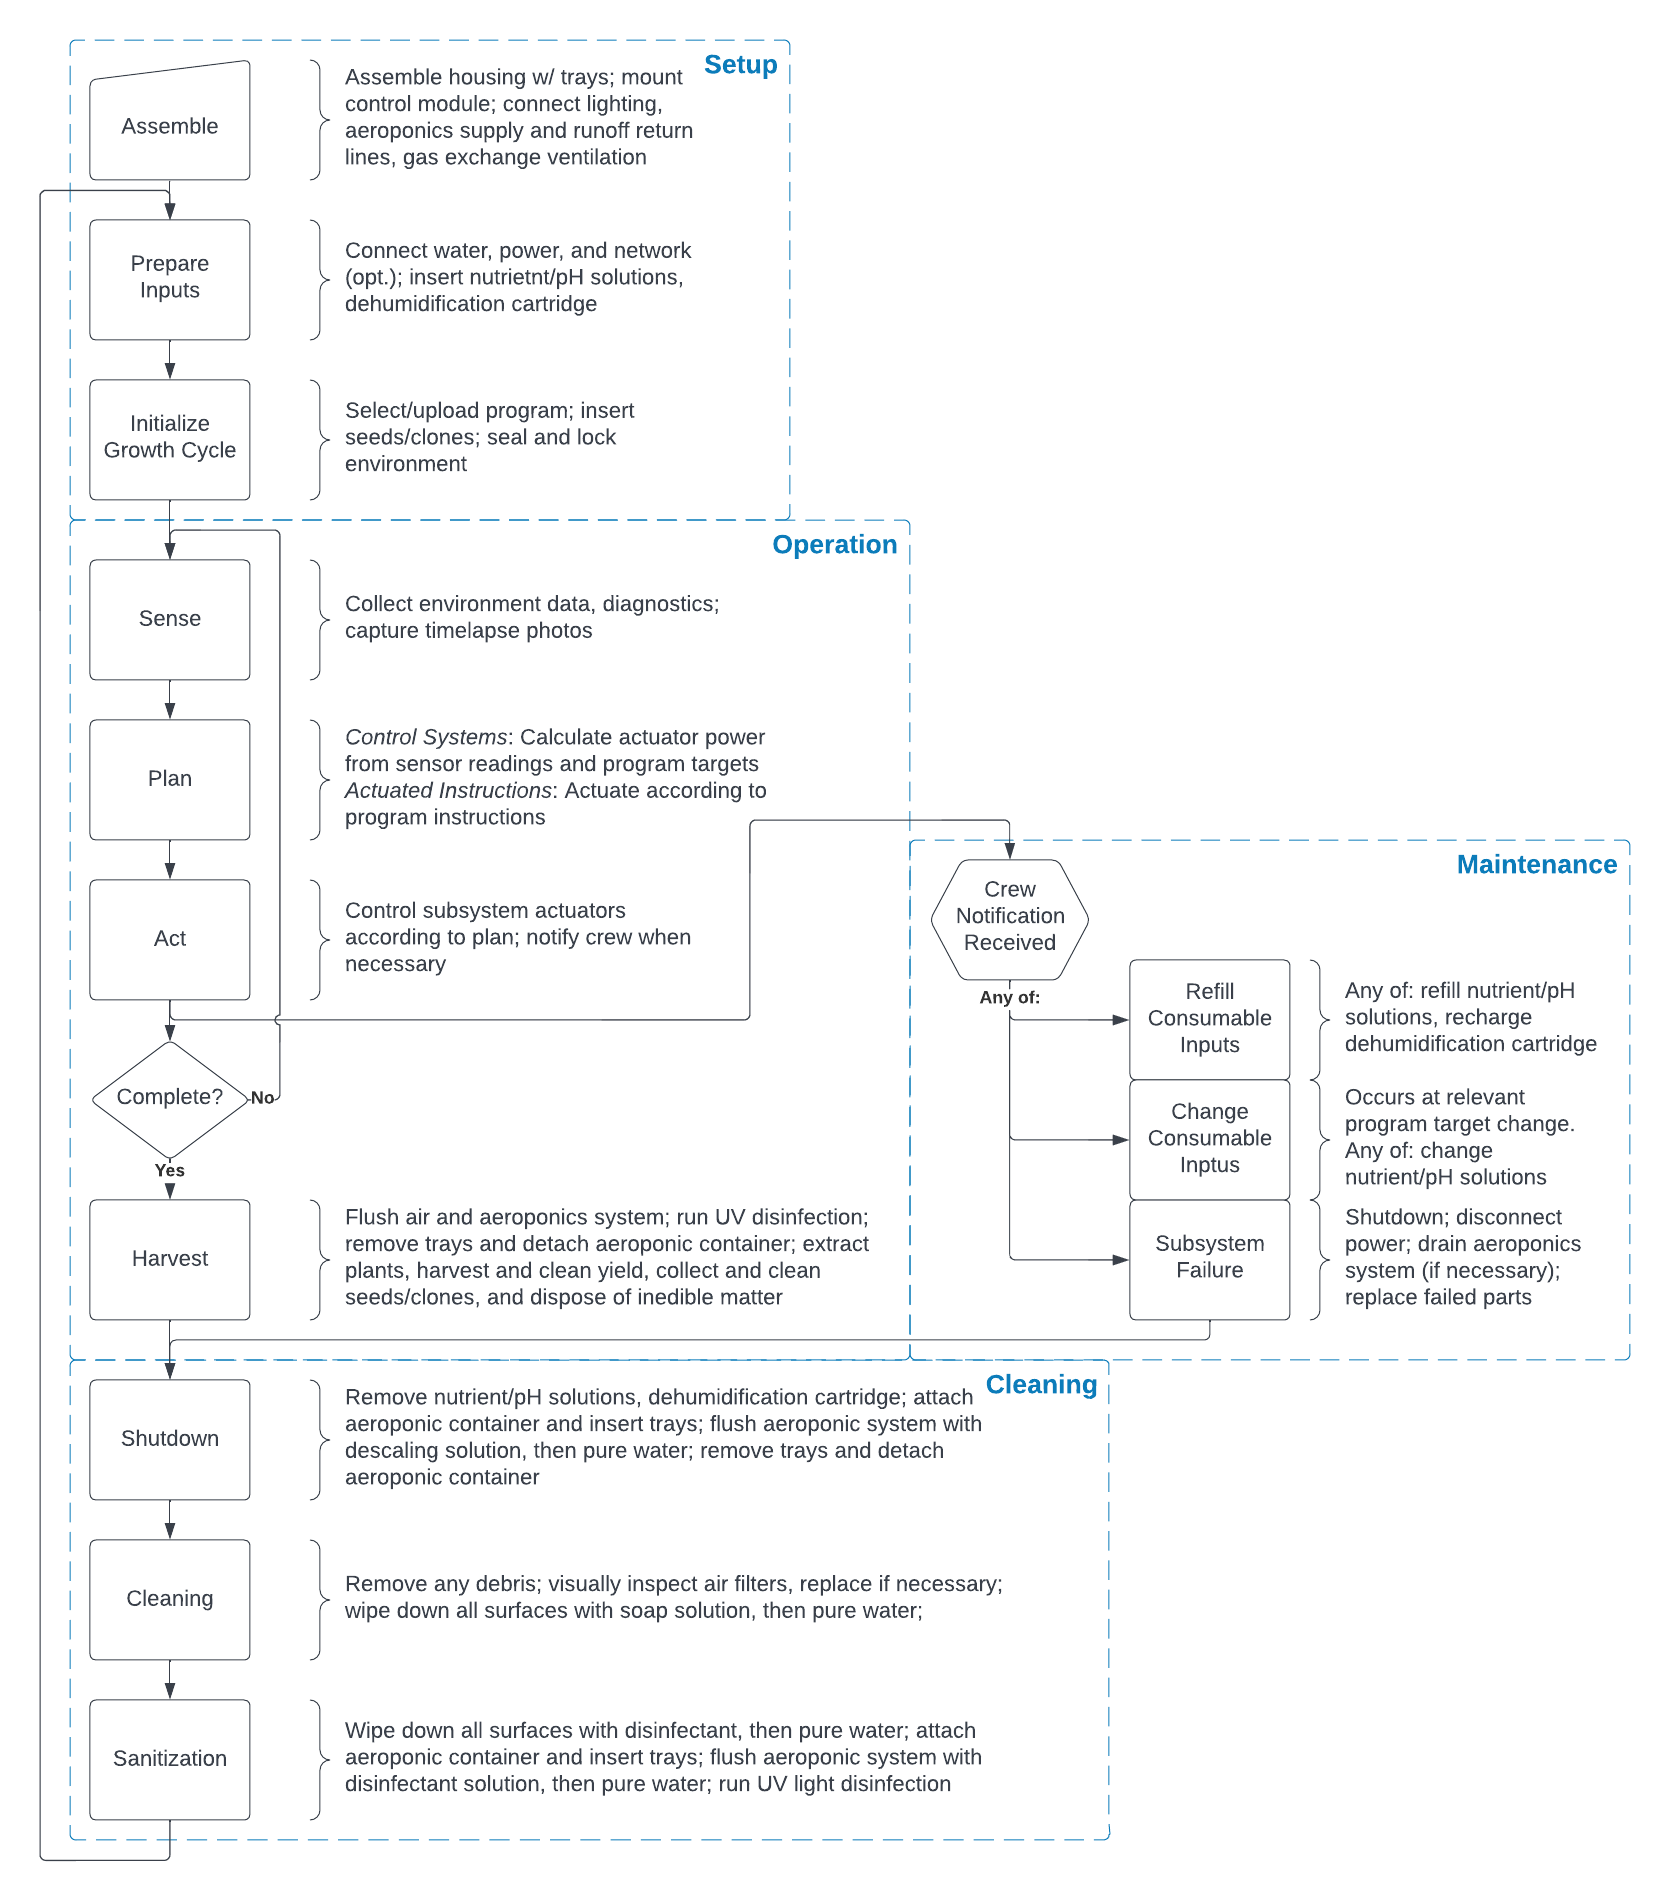
\includegraphics[width=0.9\textwidth]{../assets/figures/process.png}}
    \caption{Process diagram.}
    \label{fig:process}
\end{figure}

\clearpage

\subsubsection{Setup}
\label{sec:process_setup}

\textbf{Assembly}:
\begin{enumerate}
    \item Assemble housing, trays (see \ref{sec:housing});
    \item Mount control module, trays (see \ref{sec:housing});
    \item Connect subsystems to control module:
    \begin{itemize}
        \item \textit{Housing Solenoid Lock}: relay (see \ref{sec:housing})
        \item \textit{Aeroponics Supply \& Runoff Collection Lines}: quick-disconnect (see \ref{sec:aeroponics})
        \item \textit{Lighting Driver Board}: power, control signal (see \ref{sec:lighting})
    \end{itemize}
    \item Connect gas exchange exhaust to ventilation (see \ref{sec:gas});
\end{enumerate}

\textbf{Prepare Inputs}:
\begin{enumerate}
    \item Connect supply inputs:
    \begin{itemize}
        \item \textit{Power}: 120V 60Hz AC (see \ref{sec:automation});
        \item \textit{Network}: ethernet or wireless, optional (see \ref{sec:automation})
        \item \textit{Water}: reverse-osmosis, ambient (see \ref{sec:aeroponics})
    \end{itemize}
    \item Insert consumable inputs:
    \begin{itemize}
        \item \textit{Nutrient/pH Adjusment Solutions}: pouches (see \ref{sec:aeroponics})
        \item \textit{Dehumidification Cartridge}: recharged (see \ref{sec:dehumidification})
    \end{itemize}
\end{enumerate}

\textbf{Initialize Growth Cycle}:
\begin{enumerate}
    \item Select or upload program;
    \item Insert seeds/clones;
    \item Seal and lock environment;
    \item Start growth cycle;
\end{enumerate}

\textbf{Proceed to Operation} (see \ref{sec:process_operation}).

\subsubsection{Operation}
\label{sec:process_operation}

\textbf{Sense, Plan, Act} represent the three simultaneous automatic processes of the program's execution (see \ref{sec:automation}).

\textbf{Sense}:
Environment data, diagnostic information, and timelapse photos are captured and stored at regular intervals;

\textbf{Plan}:\\
\textit{Control Systems}: Actuator controls are calculated from sensor readings and program targets.\\
\textit{Actuated Instructions}: Actuator controls are derived from program instructions.

\textbf{Act}:
Subsystem actuators are controlled according to plan. Crew is notified to refill consumable inputs when low, change consumable inputs on program target change, and on any subsystem failure (see \ref{sec:process_maintenance}), as well as when to harvest and on End of Program (EoP).

\clearpage

\textbf{Harvest and/or EoP}:
\begin{enumerate}
    \item All air is exhausted (automatic, see \ref{sec:gas});
    \item Flush aeroponics system with pure water (automatic, see \ref{sec:aeroponics});
    \item Run UV disinfection (automatic, see \ref{sec:lighting});
    \item Unlock and open environment;
    \item Remove trays (see \ref{sec:housing}) and detach aeroponic container (see \ref{sec:aeroponics});
    \item \textbf{If EoP}: Extract plants;
    \item Harvest and clean yield;
    \item Collect, clean, and store seeds/clones;
    \item \textbf{If EoP}: Dispose of inedible matter;
\end{enumerate}

\textbf{If EoP, proceed to Cleaning} (see \ref{sec:process_cleaning})\textbf{. Otherwise, seal and lock environment and resume program.}

\subsubsection{Maintenance}
\label{sec:process_maintenance}

\textbf{Notification Handling}:
\begin{itemize}
    \item \textit{Refill Consumable Inputs}: includes refilling nutrient/pH adjustment solutions (see \ref{sec:aeroponics}), recharging the dehumidification cartridge (see \ref{sec:dehumidification})
    \item \textit{Change Consumable Inputs}: includes changing nutrient/pH adjustment solutions (see \ref{sec:aeroponics})
    \item \textit{Subsystem Failure}: all operation stopped, proceed to \textit{Shutdown} (see \ref{sec:process_cleaning}), disconnect power (see \ref{sec:automation}), then drain aeroponics system if necessary (see \ref{sec:aeroponics}) and replace failed components
\end{itemize}

\subsubsection{Cleaning}
\label{sec:process_cleaning}

\textbf{Shutdown}:
\begin{enumerate}
    \item Remove nutrient/pH solutions (see \ref{sec:aeroponics}), dehumidification cartridge (see \ref{sec:dehumidification});
    \item Attach aeroponic container (see \ref{sec:aeroponics}) and insert trays (see \ref{sec:housing});
    \item Flush aeroponic system with descaling solution (see \ref{sec:aeroponics});
    \item Flush aeroponic system with pure water (see \ref{sec:aeroponics});
    \item Remove trays (see \ref{sec:housing}) and detach aeroponic container (see \ref{sec:aeroponics});
\end{enumerate}

\textbf{Cleaning}:
\begin{enumerate}
    \item Visually inspect all surfaces for debris (remove) and components for damage (replace);
    \item Visually inspect all air filters (see \ref{sec:dehumidification}, \ref{sec:gas}), replace if necessary;
    \item Wipe down all surfaces with soap solution;
    \item Wipe down all surfaces with pure water;
\end{enumerate}

\textbf{Sanitization}:
\begin{enumerate}
    \item Wipe down all surfaces with disinfectant solution;
    \item Wipe down all surfaces with pure water;
    \item Dry all surfaces;
    \item Attach aeroponic container (see \ref{sec:aeroponics}) and insert trays (see \ref{sec:housing});
    \item Flush aeroponic system with disinfectant solution (see \ref{sec:aeroponics});
    \item Flush aeroponic system with pure water (see \ref{sec:aeroponics});
    \item Seal and lock environment;
    \item Run UV sanitization (\ref{sec:lighting});
\end{enumerate}

\textbf{Proceed to Prepare Inputs} (see \ref{sec:process_setup}).

\section{System-Level Build Process Report}
% System-level report (i.e. block diagram) of build process

\subsection{Materials}
\subsubsection{System}

\textbf{Automation}\\

\begin{table}[!h]
    \centering
    \begin{tabular}{|c|l|l|l|c|}
    \hline
        Index   & Manufacturer Part Number  & Manufacturer Name         & Description                       & Quantity  \\ \hline
        1       & A000005                   & Arduino                   & ARDUINO NANO ATMEGA328 EVAL BRD   & 1         \\ \hline
        2       & S404GSEJ6-U3000-3         & Delkin Devices, Inc.      & 4GB MLC MICROSD CARD (-25C - +85  & 1         \\ \hline
        3       & 61304021121               & Würth Elektronik          & CONN HEADER VERT 40POS 2.54MM     & 1         \\ \hline
        4       & SC0510                    & Raspberry Pi              & ZERO 2 W                          & 1         \\ \hline
        5       & DMN2005K-7                & Diodes Incorporated       & MOSFET N-CH 20V 300MA SOT23-3     & 2         \\ \hline
        6       & RC0603FR-0710KL           & YAGEO                     & RES 10K OHM 1\% 1/10W 0603        & 5         \\ \hline
        7       & 4484                      & Adafruit Industries LLC   & MINI PITFT 1.3 FOR RASPBERRY PI   & 1         \\ \hline
        8       & 5055670271                & Molex                     & CONN HEADER SMD R/A 2POS 1.25MM   & 2         \\ \hline
        9       & 5055670471                & Molex                     & CONN HEADER SMD R/A 4POS 1.25MM   & 5         \\ \hline
        10      & 5055670871                & Molex                     & CONN HEADER SMD R/A 8POS 1.25MM   & 3         \\ \hline
        11      & 5055670681                & Molex                     & CONN HEADER SMD R/A 6POS 1.25MM   & 3         \\ \hline
    \end{tabular}
    \caption{Automation system electronic components.}
    \label{tab:automation_components}
\end{table}

In addition, 1x \textit{Automation Motherboard PCB}: 2 Layers, 1 oz. Copper, 1.6mm Thickness, Suggested: HASL Finish (Lead-Free), White PCB, Black Silkscreen

\textbf{Housing}\\

\begin{table}[!ht]
    \centering
    \begin{tabular}{|l|l|c|l|l|}
    \hline
        Part                    & Description                                           & Quantity  & Supplier          & Supplier Part Number  \\ \hline
        Control Module Housing  & 5-Sided enclosure                                     & 1         & Protocase         & ~                     \\ \hline
        Frame Front X Extrusion & Silver Painted, 20x20mm, Ordered 2ft., Cut to 500mm   & 2         & McMaster-Carr     & 5537T101              \\ \hline
        Frame Door Y Extrusion  & Silver Painted, 20x20mm, Ordered 2ft., Cut to 500mm   & 2         & McMaster-Carr     & 5537T101              \\ \hline
        Frame Rear X Extrusion  & Silver Painted, 20x20mm, Ordered 2ft., Cut to 460mm   & 2         & McMaster-Carr     & 5537T101              \\ \hline
        Frame Door X Extrusion  & Silver Painted, 20x20mm, Ordered 2ft., Cut to 460mm   & 2         & McMaster-Carr     & 5537T101              \\ \hline
        Frame Rear Y Extrusion  & Silver Painted, 20x40mm, Ordered 2ft., Cut to 460mm   & 2         & McMaster-Carr     & 5537T111              \\ \hline
        Frame Front Y           & Silver Painted, 20x20mm, Ordered 2ft., Cut to 460mm   & 2         & McMaster-Carr     & 5537T101              \\ \hline
        Frame Z                 & Silver Painted, 20x20mm, Ordered 2ft., Cut to 460mm   & 4         & McMaster-Carr     & 5537T101              \\ \hline
        Tray X Extrusion        & Silver Painted, 20x20mm, Ordered 2ft., Cut to 440mm   & 4         & McMaster-Carr     & 5537T101              \\ \hline
        Tray Z Extrusion        & Silver Painted, 20x20mm, Ordered 2ft., Cut to 400mm   & 6         & McMaster-Carr     & 5537T101              \\ \hline
        Nozzle Arm Extrusion    & Silver Painted, 20x20mm, Ordered 1ft., Cut to 150mm   & 2         & McMaster-Carr     & 5537T101              \\ \hline
        M5x0.8 10mm Bolts       & Alloy Steel, Black Oxide Coated, Socket Head Cap      & 139       & McMaster-Carr     & 91290A224             \\ \hline
        M5x0.8 16mm Bolts       & Alloy Steel, Black Oxide Coated, Socket Head Cap      & 10        & McMaster-Carr     & 91290A232             \\ \hline
        M4x0.7 16mm Bolts       & Alloy Steel, Black Oxide Coated, Socket Head Cap      & 12        & McMaster-Carr     & 91290A154             \\ \hline
        M4x0.7 Hex Nuts         & High-Strength Steel, Black Oxide Coated               & 12        & McMaster-Carr     & 94166A110             \\ \hline
        M5 T-Nuts               & Zinc-Plated Steel, Black Painted, for 5mm Slot        & 139       & McMaster-Carr     & 5537T651              \\ \hline
        M5x0.8 Hex Nuts         & Alloy Steel, Black Oxide Coated                       & 10        & McMaster-Carr     & 94166A120             \\ \hline
        Foam Insulation         & DUROSPAN GPS R5 4ft. x 8ft. x 1in.                    & 1         & Home Depot Canada & 1001211234            \\ \hline
        Reflective Mylar        & 27in. x 12ft. x 0.002in., Aluminum-coated PET         & 1         & McMaster-Carr     & 7538T11               \\ \hline
        Adhesive                & LePage PL300 Foamboard 295mL                          & 2         & Home Depot Canada & 1000403469            \\ \hline
        Grow Cup                & 2in. Diameter                                         & 16        & Amazon            & ~                     \\ \hline
        Door Hinges             & Plastic, Black, for 20x20mm Extrusion                 & 2         & McMaster-Carr     & 5537T85               \\ \hline
        Feet Bumpers            & Adhesive-Back, Medium-Hard Polyurethane, Black        & 4         & McMaster-Carr     & 95495K24              \\ \hline
    \end{tabular}
    \caption{Housing subsystem components.}
    \label{tab:housing_parts}
\end{table}

\begin{table}[!ht]
    \centering
    \begin{tabular}{|l|c|l|l|}
    \hline
        Part                        & Quantity  & Materials             & Process           \\ \hline
        L Bracket                   & 12        & PETG Filament         & 3D Printing       \\ \hline
        L Bracket (Grow Tray)       & 4         & PETG Filament         & 3D Printing       \\ \hline
        Diagonal Bracket            & 4         & PETG Filament         & 3D Printing       \\ \hline
        T Bracket                   & 10        & PETG Filament         & 3D Printing       \\ \hline
        Tray Hook BL                & 2         & PETG Filament         & 3D Printing       \\ \hline
        Tray Hook BR                & 2         & PETG Filament         & 3D Printing       \\ \hline
        Tray Hook FL                & 2         & PETG Filament         & 3D Printing       \\ \hline
        Tray Hook FR                & 2         & PETG Filament         & 3D Printing       \\ \hline
        Grow Plate Quarters         & 4         & 210x210x5mm PET Sheet & Table Saw         \\ \hline
        Grow Plate Washer           & 1         & PETG Filament         & 3D Printing       \\ \hline
        Nozzle Mount A              & 2         & PETG Filament         & 3D Printing       \\ \hline
        Nozzle Mount B              & 2         & PETG Filament         & 3D Printing       \\ \hline
        Lighting LED Board Mount    & 5         & PETG Filament         & 3D Printing       \\ \hline
        Lighting Power Board Mount  & 1         & PETG Filament         & 3D Printing       \\ \hline
        Feet                        & 4         & PETG Filament         & 3D Printing       \\ \hline
    \end{tabular}
    \caption{Housing subsystem fabricated parts.}
    \label{tab:housing_fabrication}
\end{table}

\textbf{Aeroponics}\\


\textbf{Leaf-Zone Thermoregulation}\\


\textbf{Humidification}\\


\textbf{Dehumidification}\\


\textbf{Gas Composition Regulation and Exchange}\\


\textbf{Lighting}\\


\subsubsection{Inputs}
% Supply inputs (water, power, network), consumable inputs (pH/nutrient solutions, dehumidification cartridge)

\textbf{Supply Inputs}
\begin{itemize}
    \item \textit{Water}: reverse-osmosis, ambient
    \item \textit{Power}: 120V 60Hz AC\footnote{The power supply can be altered to suit a variety of power inputs (i.e. DC)}
    \item \textit{Network}: ethernet or wireless, optional
\end{itemize}

\textbf{Consumable Inputs}
\begin{itemize}
    \item \textit{Nutrient/pH Adjusment Solutions}: pouches
    \item \textit{Dehumidification Cartridge}: recharged
\end{itemize}

\subsubsection{Outputs}
% Food outputs(?), by-products/waste (waste water from flushing, dehumidification cartridge)

\textbf{Food Outputs}\\


\textbf{By-Products \& Waste}\\


\subsubsection{Maintenance}

\textbf{Spare Components}\\


\textbf{Tools}\\


\subsubsection{Cleaning}

\textbf{Soaps}\\


\textbf{Disinfectants}\\


\textbf{Tools}\\



\section{Prototype Build Status}
% SPECIFICALLY build status - from functional prototyping to testing to refinement
\subsection{Automation Subsystem}
\subsection{Housing}
\subsection{Aeroponic Subsystem}
\subsubsection{Solution Nutrients and pH Regulation}
\subsubsection{Solution/Root-Zone Temperature Regulation}
\subsubsection{Mist Delivery}
\subsection{Leaf-Zone Thermoregulation Subsystem}
\subsection{Leaf-Zone Humidity Regulation Subsystem}
\subsubsection{Leaf-Zone Humidification}
\subsubsection{Leaf-Zone Dehumidification}
\subsection{Gas Composition Regulation Subsystem}
\subsubsection{Gas Exchange}
\subsubsection{Gas Supplementation}
\subsection{Lighting}

\section{Prototyping Summary}
% What's going well? What's proving to be challenging?
% Evidence (videos, photographs, diagrams, etc.)

\section{Development Timeline}
% Incl. estimated completion date

\section{Preliminary Results}
% Predicted and/or produced

\newpage

% References
\bibliographystyle{IEEEtran}
\bibliography{references}
\end{document}